\chapter{Analyse - Befragung}\label{analyse_umfrage}

\paragraph{Frage 1} Die aktuelle Lösung entspricht insgesamt meinem Bedarf. \\ 


\noindent Stimme gar nicht zu { }{ } O 1 { }{ } O 2 { }{ } O 3 { }{ } O 4 { }{ } O 5 { }{ } Stimme völlig zu \\


\noindent Die durchschnittliche Antwort lag hier bei: 3. \\


\paragraph{Frage 2} Ich fühlte mich sehr vertraut bei dem Umgang mit der vorgestellten Lösung. \\ 


\noindent Stimme gar nicht zu { }{ } O 1 { }{ } O 2 { }{ } O 3 { }{ } O 4 { }{ } O 5 { }{ } Stimme völlig zu \\


\noindent Die durchschnittliche Antwort lag hier bei: 3. \\


\paragraph{Frage 3} Es ist einfach, die gewünschten Informationen zu finden. \\ 


\noindent Stimme gar nicht zu { }{ } O 1 { }{ } O 2 { }{ } O 3 { }{ } O 4 { }{ } O 5 { }{ } Stimme völlig zu \\


\noindent Die durchschnittliche Antwort lag hier bei: 2. \\


\paragraph{Frage 4} Die aktuelle Lösung ist optisch ansprechend. \\ 


\noindent Stimme gar nicht zu { }{ } O 1 { }{ } O 2 { }{ } O 3 { }{ } O 4 { }{ } O 5 { }{ } Stimme völlig zu \\


\noindent Die durchschnittliche Antwort lag hier bei: 1. \\


\paragraph{Frage 5} Die Darstellung der Informationen entspricht den Anforderungen. \\ 


\noindent Stimme gar nicht zu { }{ } O 1 { }{ } O 2 { }{ } O 3 { }{ } O 4 { }{ } O 5 { }{ } Stimme völlig zu \\


\noindent Die durchschnittliche Antwort lag hier bei: 1. \\


\paragraph{Frage 6} Die aktuelle Lösung ist sehr umständlich zu benutzen. \\ 


\noindent Stimme gar nicht zu { }{ } O 1 { }{ } O 2 { }{ } O 3 { }{ } O 4 { }{ } O 5 { }{ } Stimme völlig zu \\


\noindent Die durchschnittliche Antwort lag hier bei: 2. \\


\paragraph{Frage 7} Andere Nutzergruppen können die aktuelle Lösung problemlos bedienen. \\ 


\noindent Stimme gar nicht zu { }{ } O 1 { }{ } O 2 { }{ } O 3 { }{ } O 4 { }{ } O 5 { }{ } Stimme völlig zu \\


\noindent Die durchschnittliche Antwort lag hier bei: 2. \\


\paragraph{Frage 8} Zur Nutzung der Lösung besteht der Bedarf einer intensiven Einarbeitung. \\ 


\noindent Stimme gar nicht zu { }{ } O 1 { }{ } O 2 { }{ } O 3 { }{ } O 4 { }{ } O 5 { }{ } Stimme völlig zu \\


\noindent Die durchschnittliche Antwort lag hier bei: 4. \\


\paragraph{Frage 9} Wie gehen Sie bei der Nutzung der Lösung vor? \\ 


\noindent  Die facettierte Suche wird nicht verwendet. Es wird eher die ganze Liste an Softwareprodukte verwendet, um von dort zu ein bestimmtes Softwareprodukt zu kommen.\\


\paragraph{Frage 10} Sind Sie bei der Nutzung der aktuellen Lösung über Probleme gestolpert? Wenn ja, welche? \\ 


\noindent  Zu wenige und unnötige Informationen auf der Ergebnisseite.\\


\paragraph{Frage 11} Was könnte sich an der aktuellen Lösung verbessern? \\ 


\noindent Die Darstellung der Informationen. Nutzer*innen sollen nicht mehr zum RickView weitergeleitet werden.  \\


\paragraph{Frage 12} Welche Funktionen finden Sie sinnvoll und welche nicht sinnvoll? \\ 


\noindent Hier wurde beantwortet, dass alle Funktionen sinnvoll sind. Diese sollen aber in ihrer Darstellung verbessert werden. \\


\paragraph{Frage 14} Was könnte potenzielle Nutzer davon abhalten, dieses Produkt zu nutzen? \\ 


\noindent  Der Absprung in RickView.\\

\chapter{Konzeption - Wireframes, erste Iteration}\label{app_wireframes}

\begin{figure}[ht]
	\centering
    	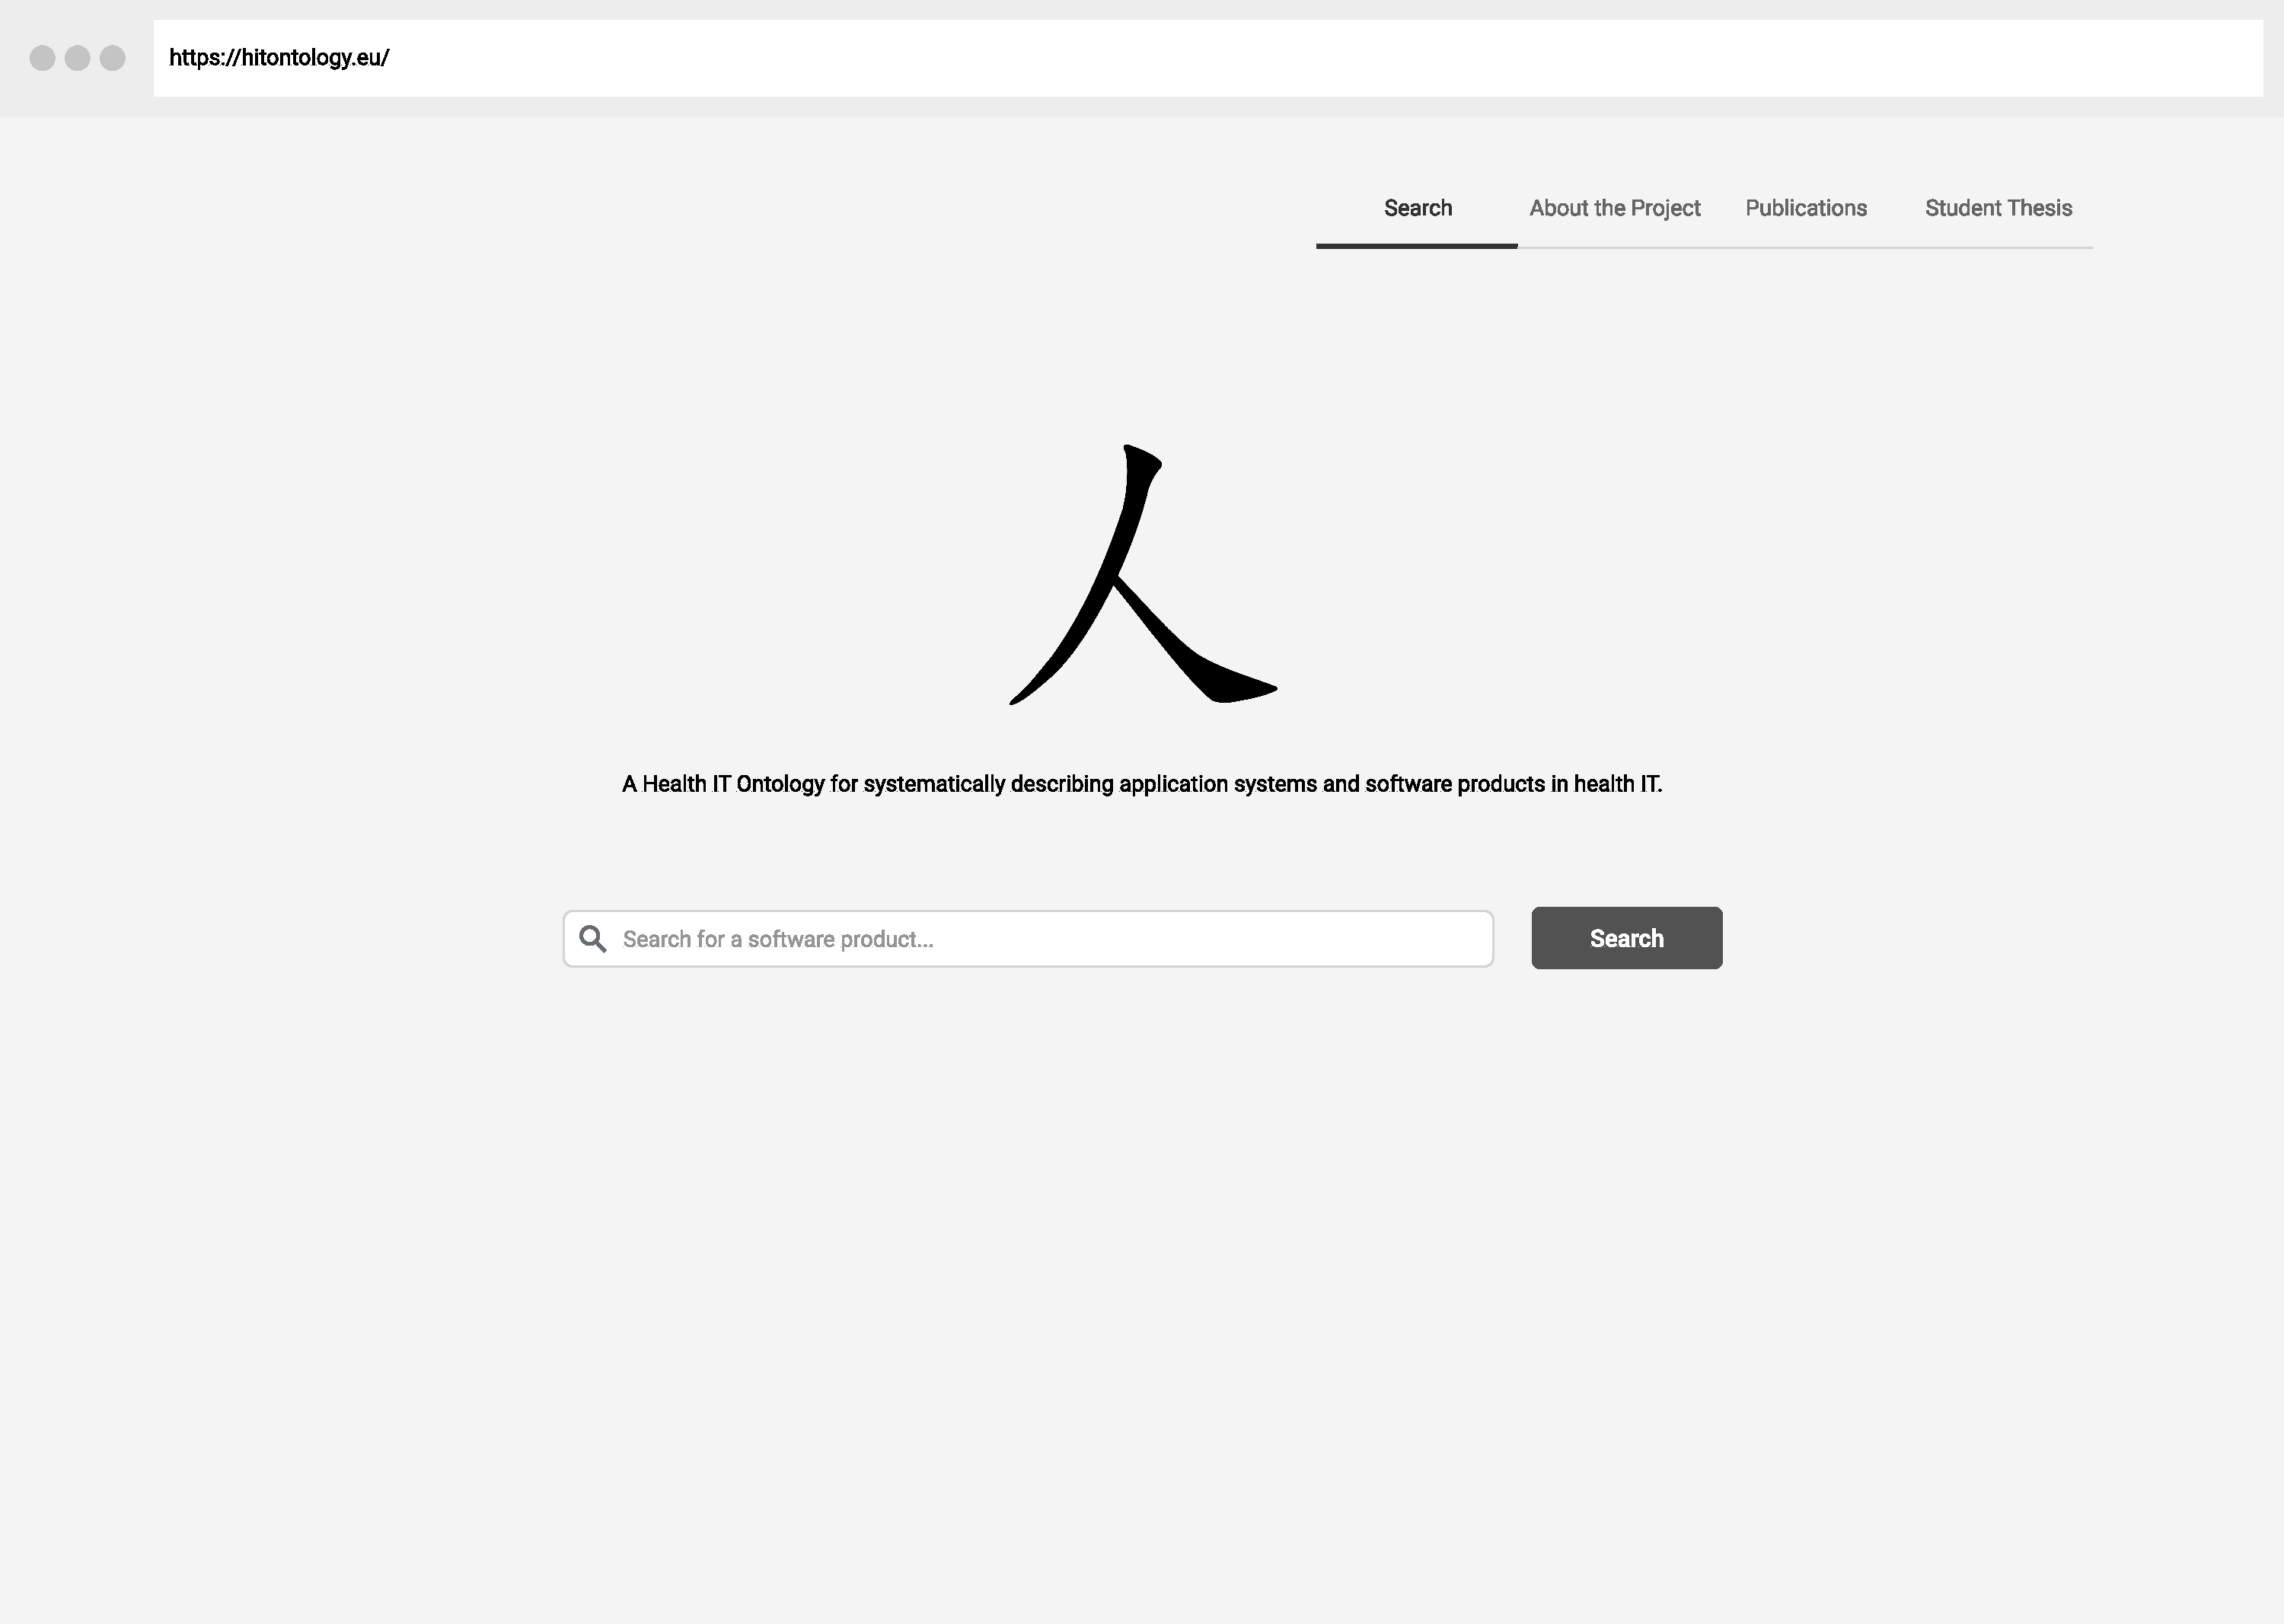
\includegraphics[width=1.4\textwidth, angle=90]{Images/Desktop_1}
   	\caption[Wireframe -- Startseite]{Wireframe Startseite -- Iteration 1}
\end{figure}

\clearpage

\begin{figure}[ht]
	\centering
    	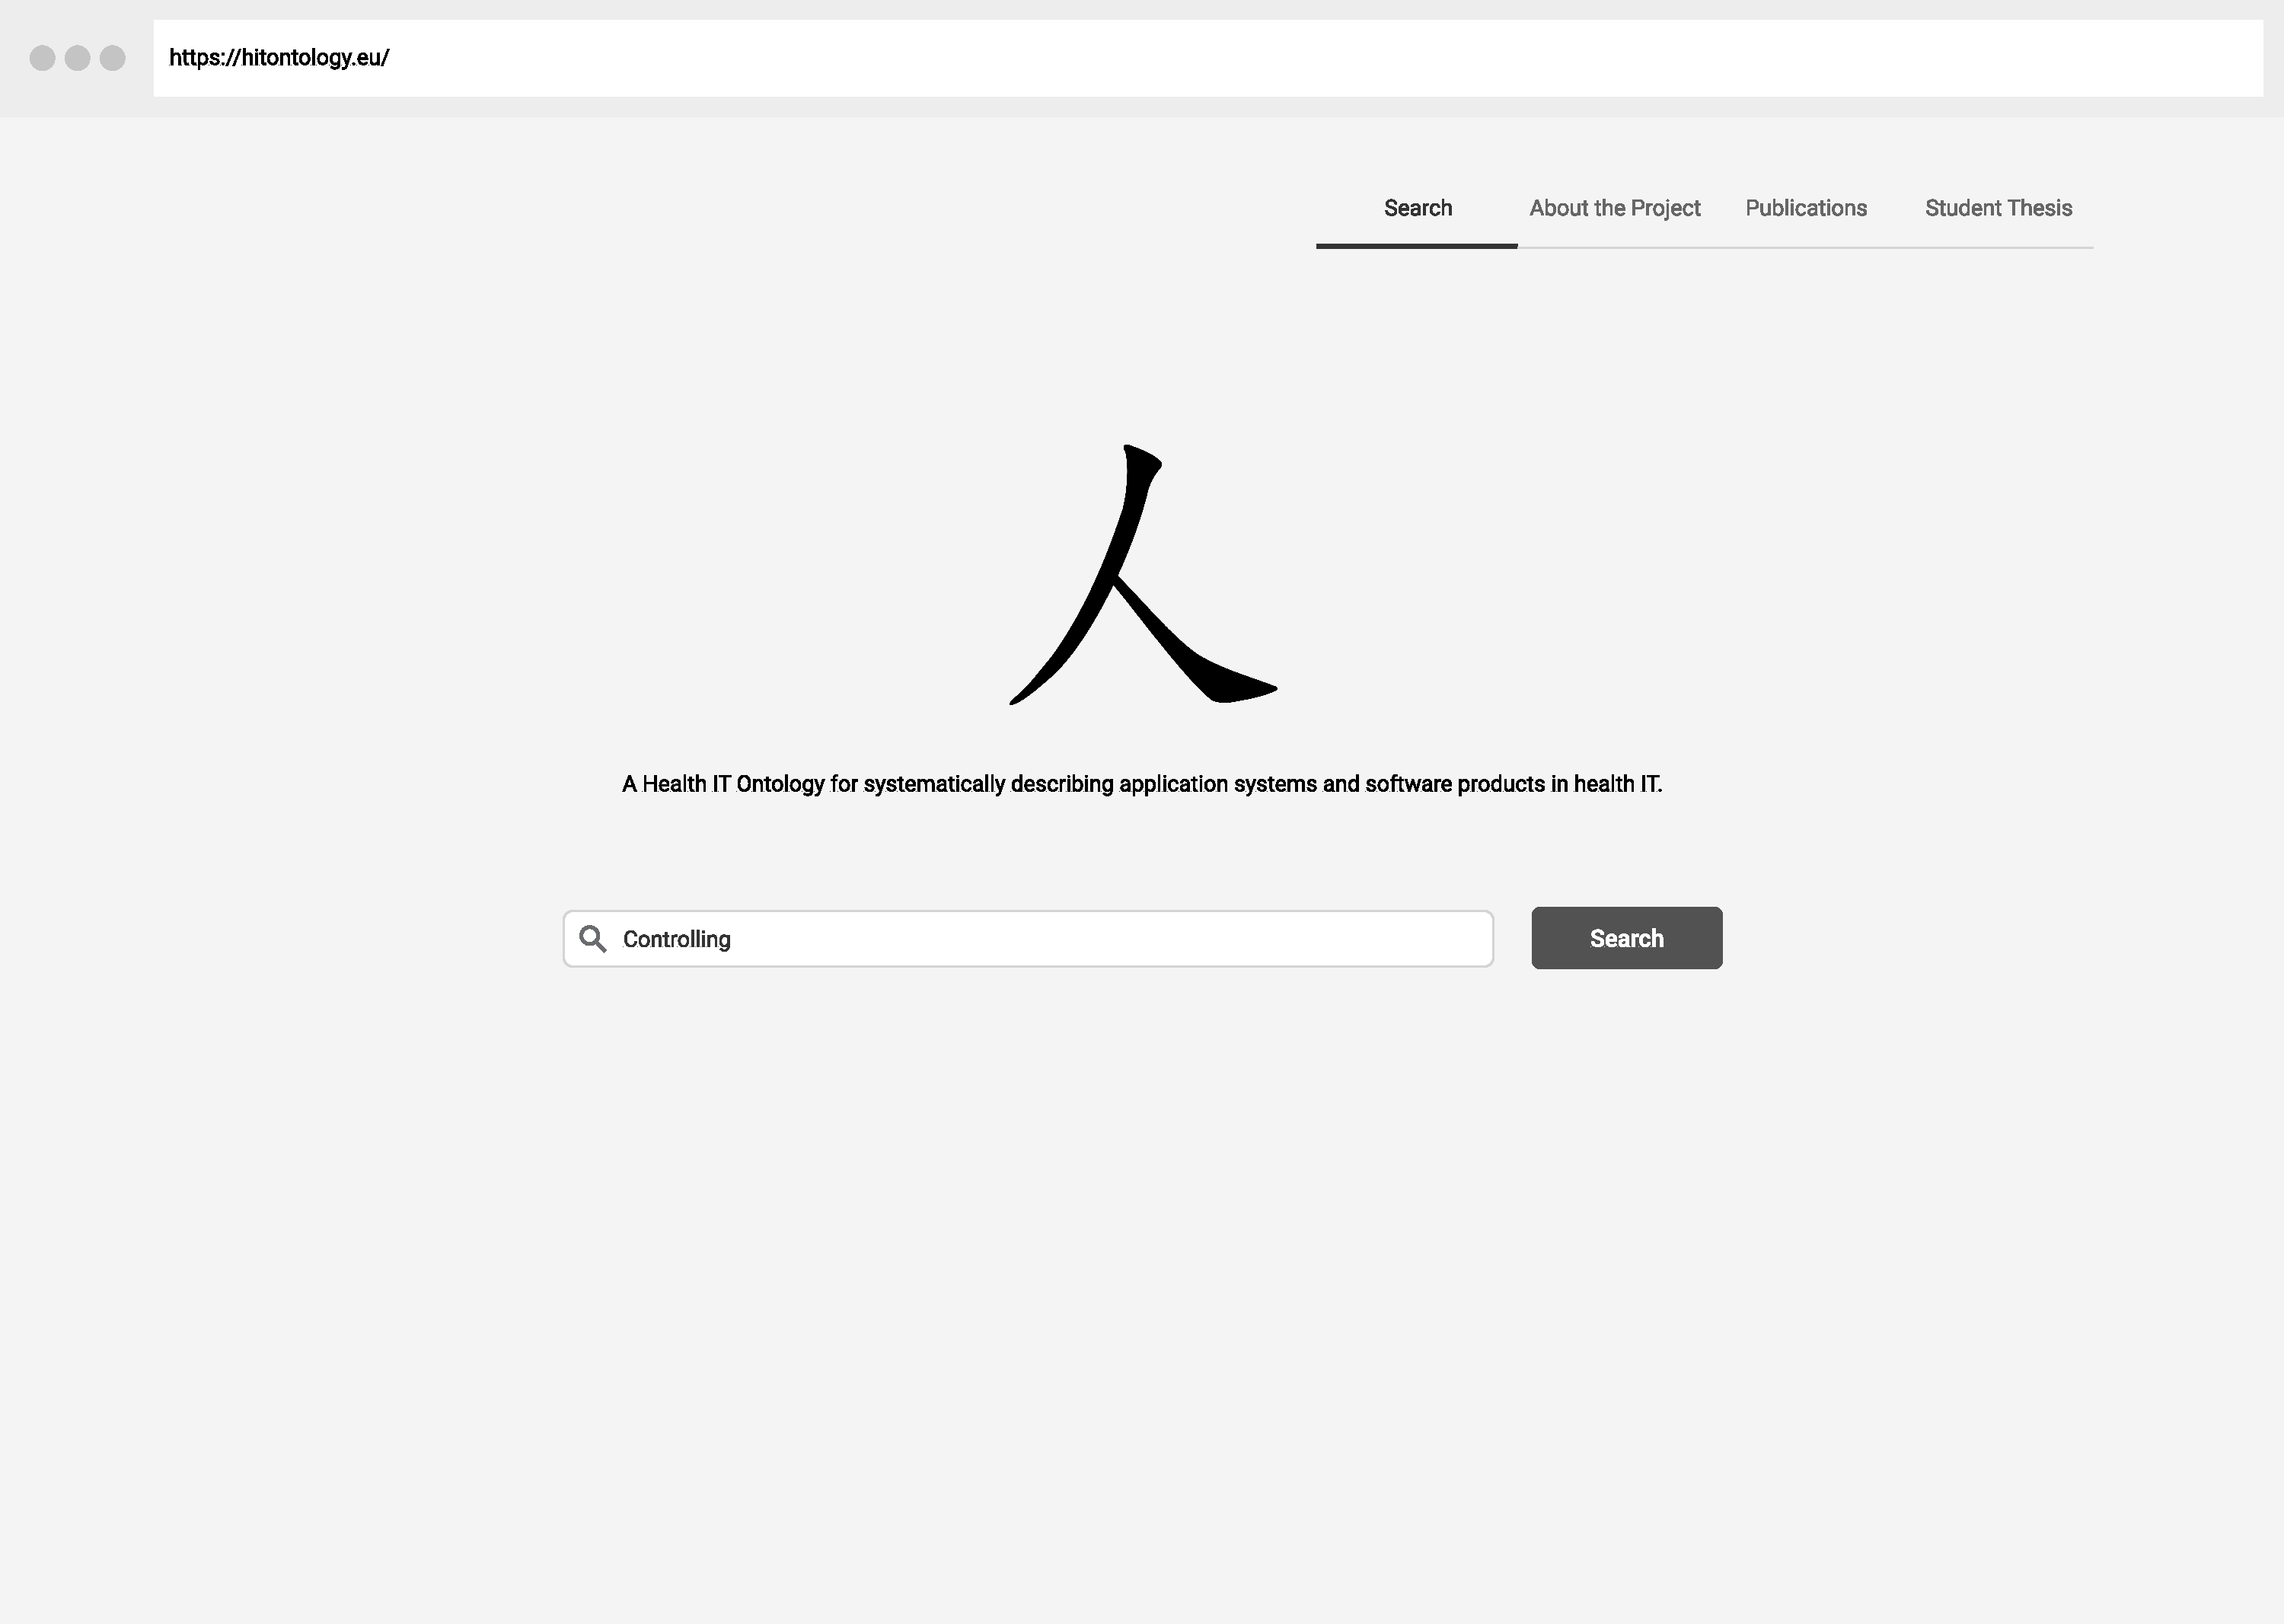
\includegraphics[width=1.4\textwidth, angle=-90]{Images/Desktop_2}
   	\caption[Wireframe -- Startseite mit aktiver Suche]{Wireframe Startseite mit aktiver Suche -- Iteration 1}
\end{figure}

\clearpage

\begin{figure}[ht]
	\centering
    	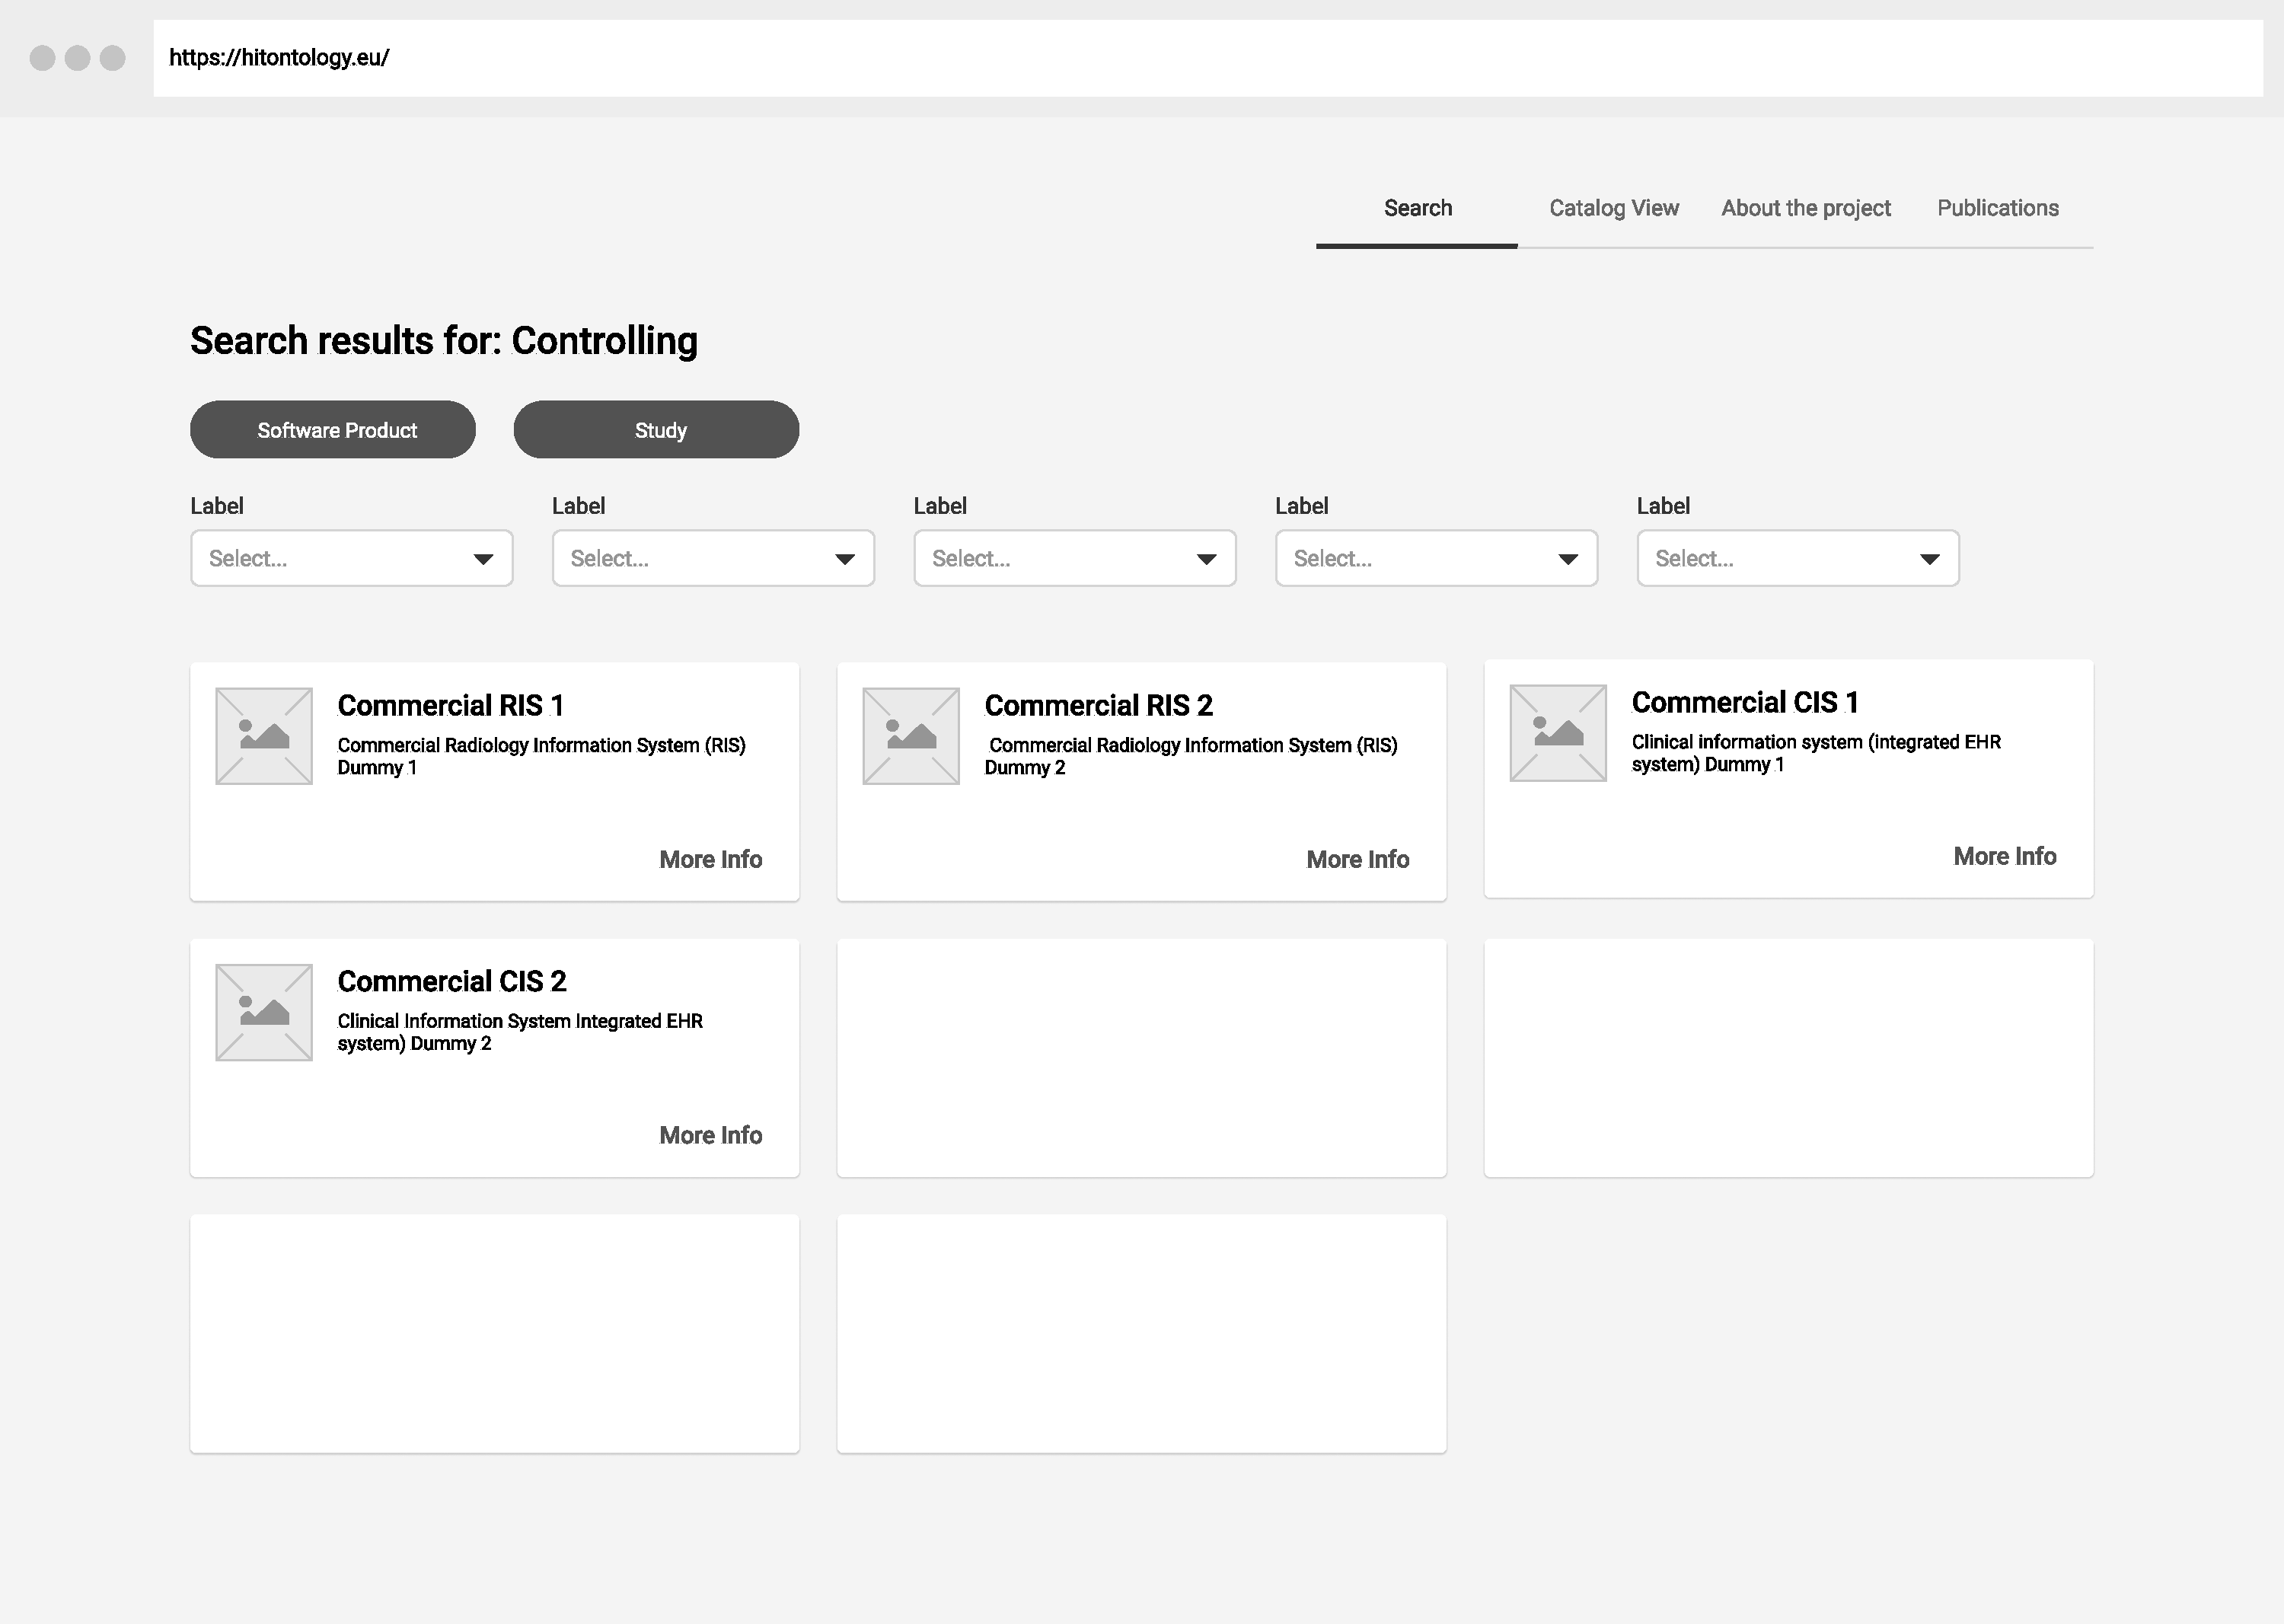
\includegraphics[width=1.4\textwidth, angle=90]{Images/Desktop_3}
   	\caption[Wireframe -- Ergebnisseite]{Wireframe Ergebnisseite -- Iteration 1}
\end{figure}

\clearpage

\begin{figure}[ht]
	\centering
    	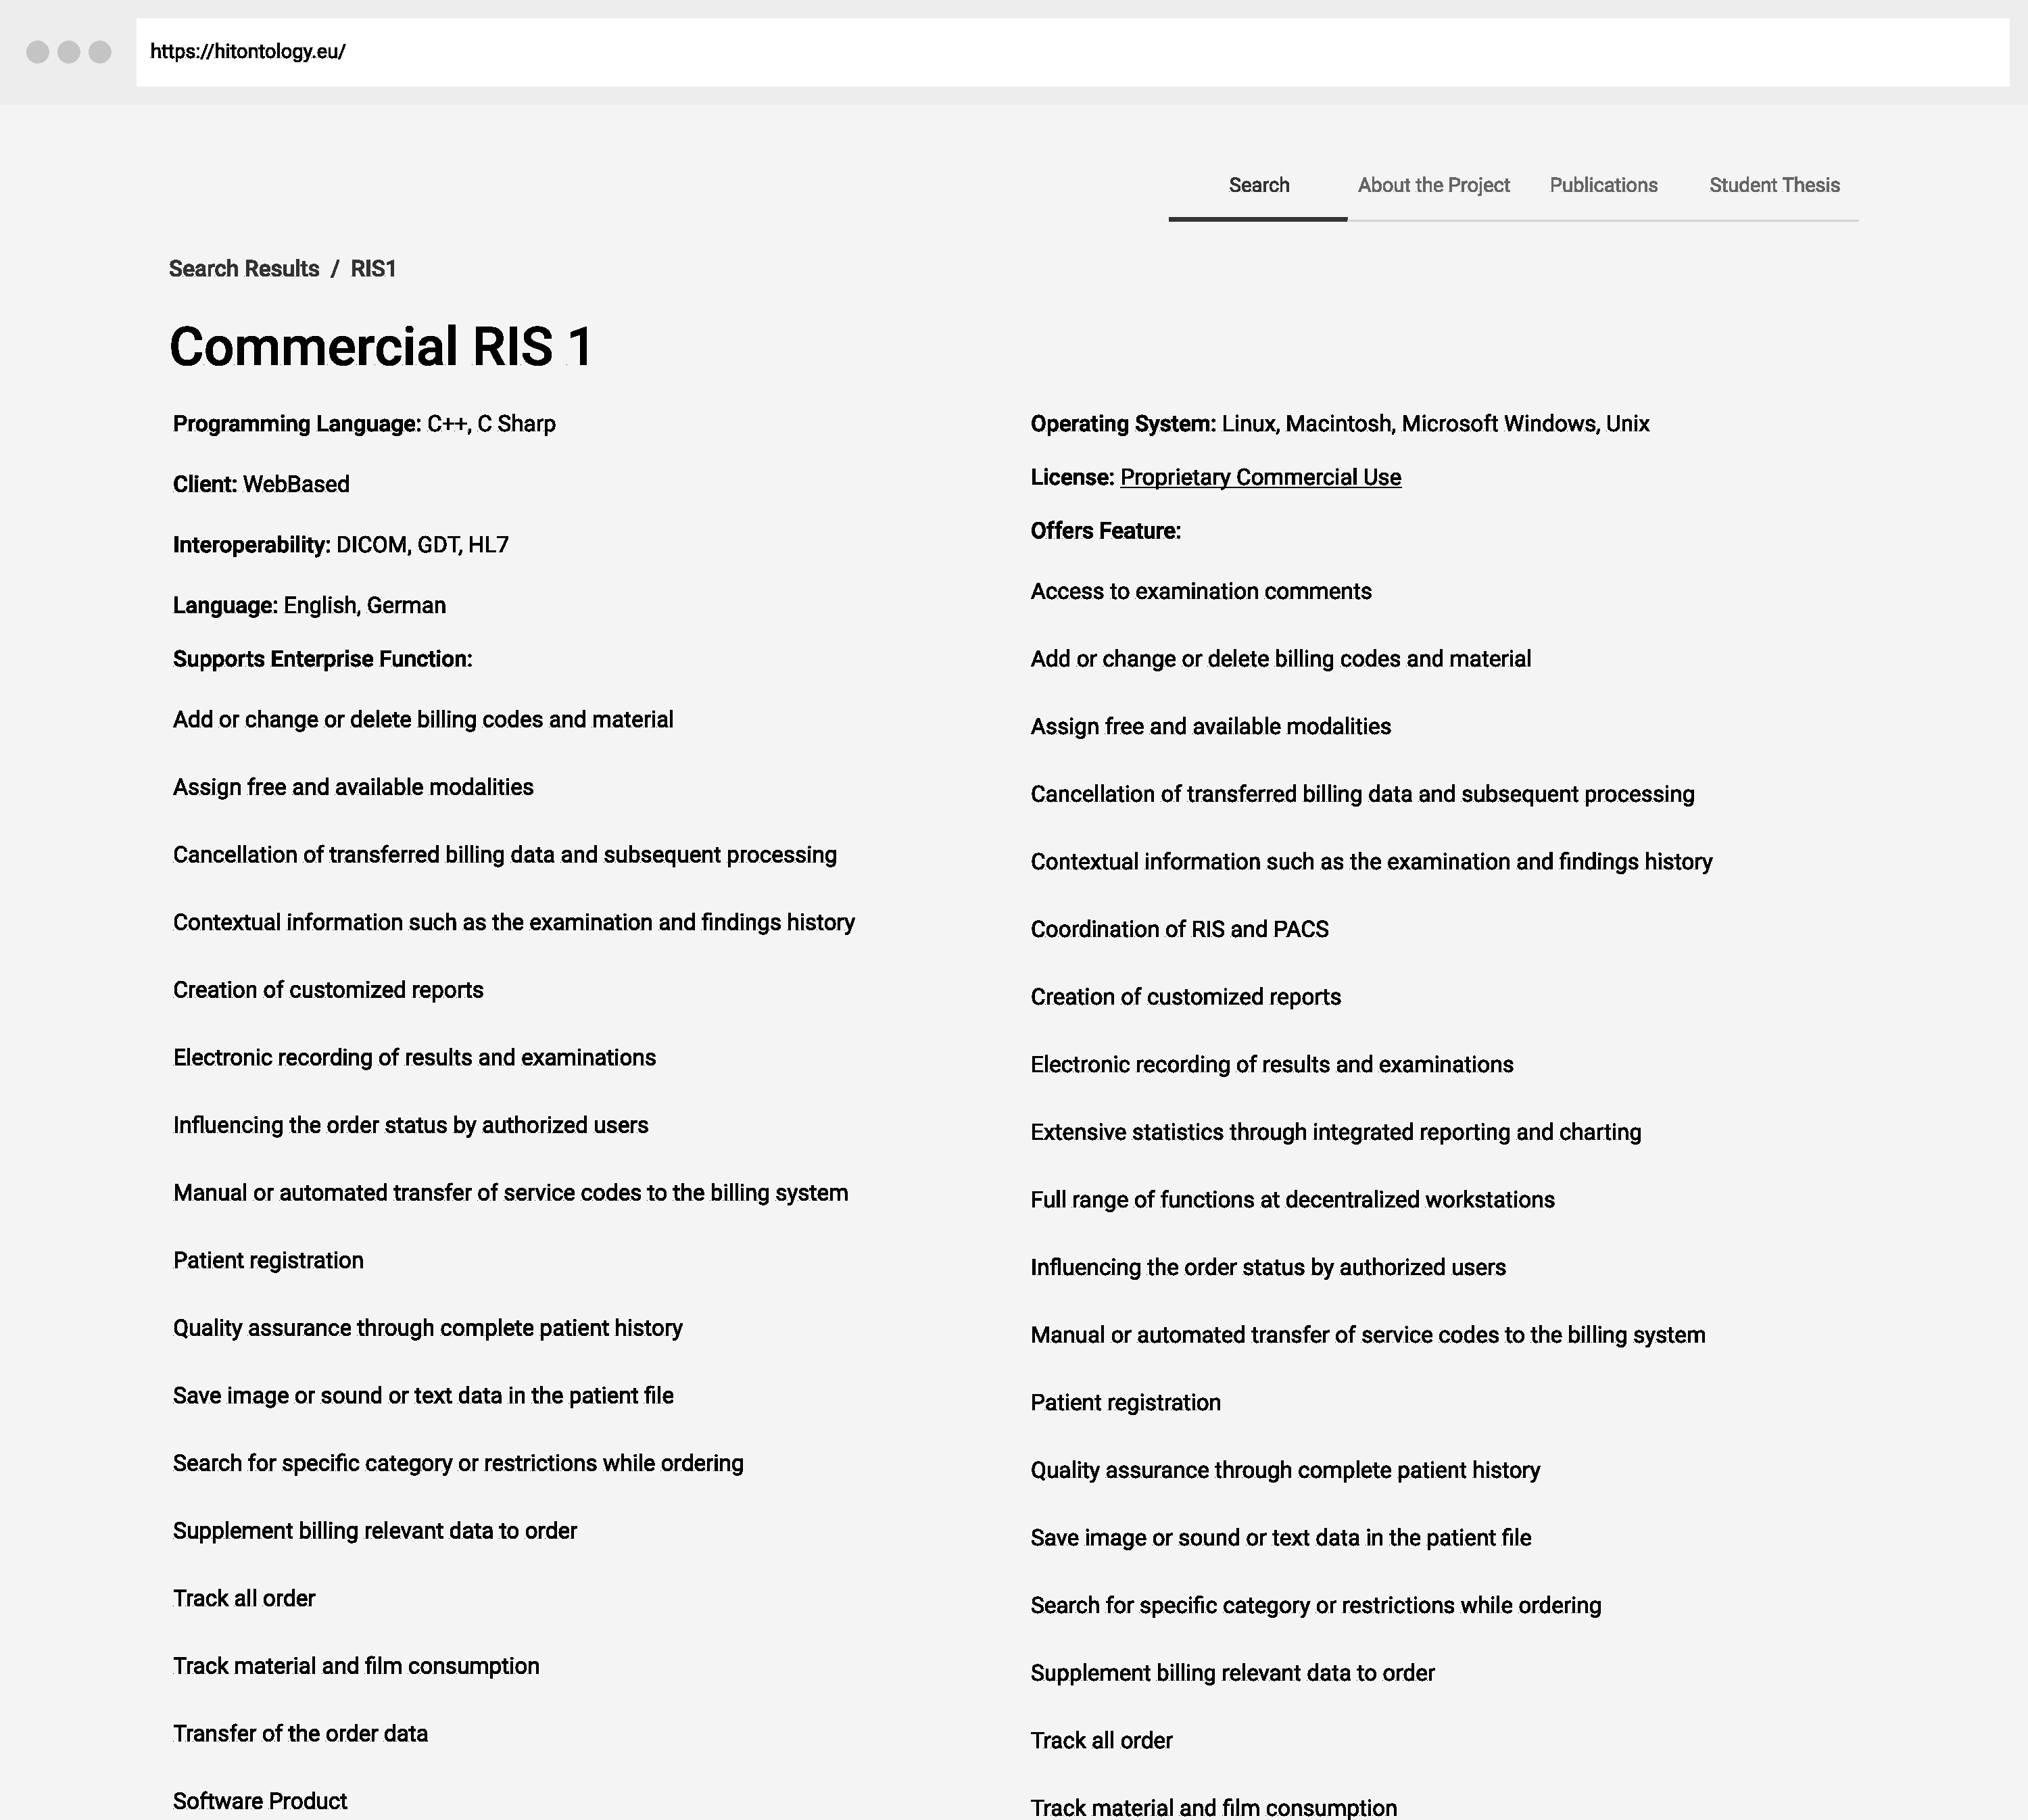
\includegraphics[width=1\textwidth]{Images/Desktop_4}
   	\caption[Wireframe -- Detailseite Softwareprodukt]{Wireframe Detailseite Softwareprodukt -- Iteration 1}
\end{figure}
